\Testart{Skript}
\Klasse{10}
\Fach{Informatik}
\Titel{Datenbanken}

\renewcommand{\Content}{
    
    \mysession{Alles}{
        \Hefteintrag{1.8}{Tabellenbeziehungen: Fremdschlüssel}{ \Large
Wenn Datensätze mittels Primärschlüssel in einer anderen Tabelle verwendet werden, spricht man dort von einem Fremdschlüssel. Im Tabellenschema werden die \LoesungLuecke{Fremdschlüssel}{8cm} durch (\hspace{8cm}) (manchmal auch \hspace{8cm}) markiert. Ein Beispiel in SQL-Island ist der Häuptling eines Dorfes, der in der Tabelle Dorf mittels bewohnernr eingetragen wird. Die \emphBlue{bewohnernr} ist hierbei \emphBlue{\LoesungLuecke{}{8cm}} in der \emphBlue{Tabelle Bewohner} und \emphGreen{\LoesungLuecke{}{8cm}} in der \emphGreen{Tabelle Dorf} (heißt hier aber \emphGreen{haeuptling}).

}



        \Hefteintrag{1}{Tabellenbeziehungen im Klassendiagramm}{

\vspace{4cm}

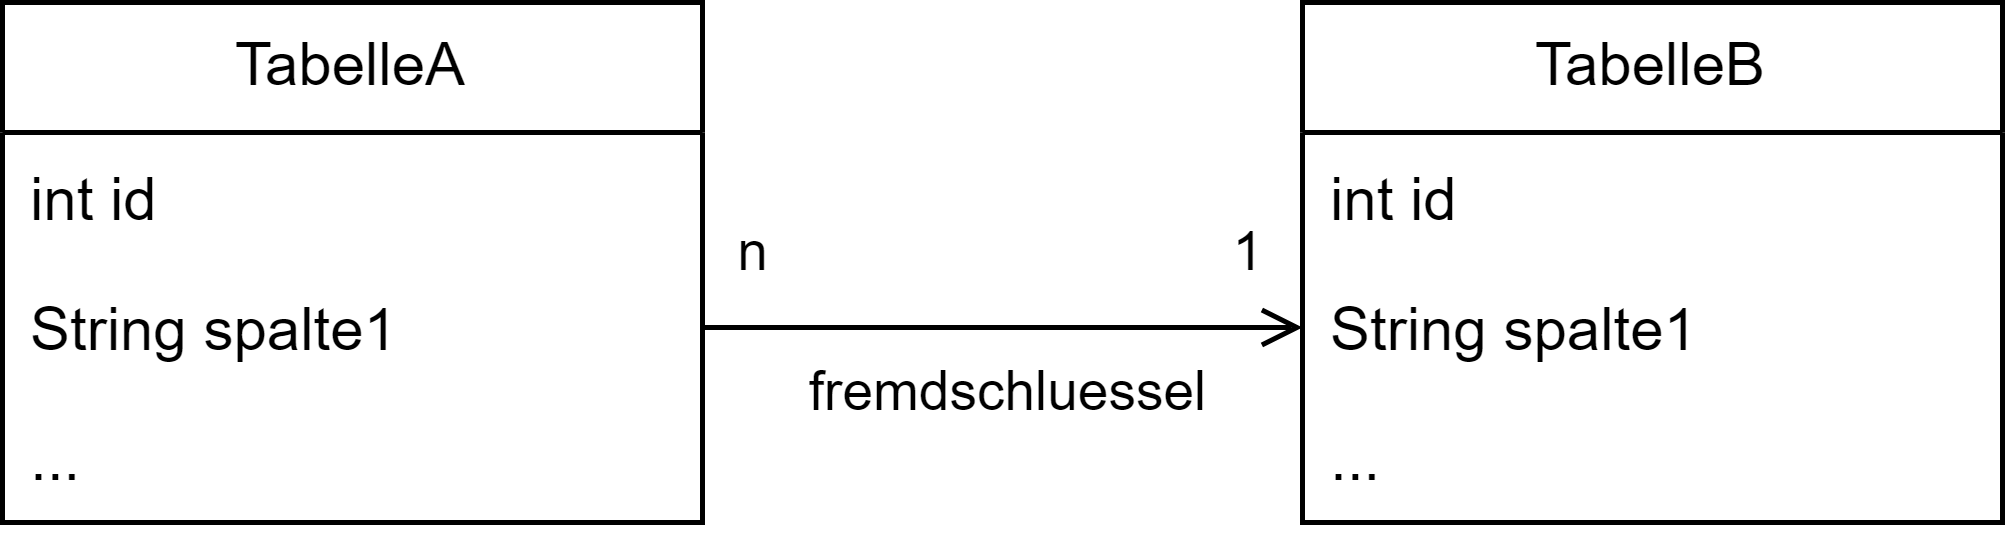
\includegraphics[width=\textwidth]{Aufgaben/img/SchemaBeziehung.png}

\vspace{4cm}
}



        \input{_Aufgaben/H02_Kardinalität}

        \Hefteintrag{2}{Kreuzprodukt / Join}{
Möchte man Daten aus zwei Tabellen mit Beziehung zueinander abfragen, gibt man beide Tabellen \emphOrange{mit Komma getrennt nach FROM} an.

Die SQL-Abfrage bildet dann das \LoesungLuecke{Kreuzprodukt}{7cm} der Tabellen. Die Ergebnistabelle enthält \LoesungLuecke{alle Kombinationen}{7cm} von Datensätzen beider Tabellen \emphOrange{(Merkregel: \LoesungLuecke{Jeder mit Jedem}{9cm})}.

Um nur zusammengehörige Datensätze (also solche, die miteinenader in Beziehung stehen, z.B. eine Bewohner mit seinem Dorf) auszuwählen, ergänzt man als \emphGreen{Selektion} eine \emphGreen{Gleichheitsbedingung} zwischen Fremd- und zugehörigem \LoesungLuecke{Primärschlüssel}{8cm}. Dann spricht man von einem \LoesungLuecke{Join}{4cm}.

Zum Beispiel kann man in SQL-Island die Daten aller Dörfer und ihrer zugehörigen Häuptlinge so ausgeben:



\begin{center}
SELECT * \\\emphOrange{FROM Dorf, Bewohner} \\\emphGreen{WHERE Dorf.haeuptling = Bewohner.bewohnernr}    
\end{center}
}


        \begin{center}
    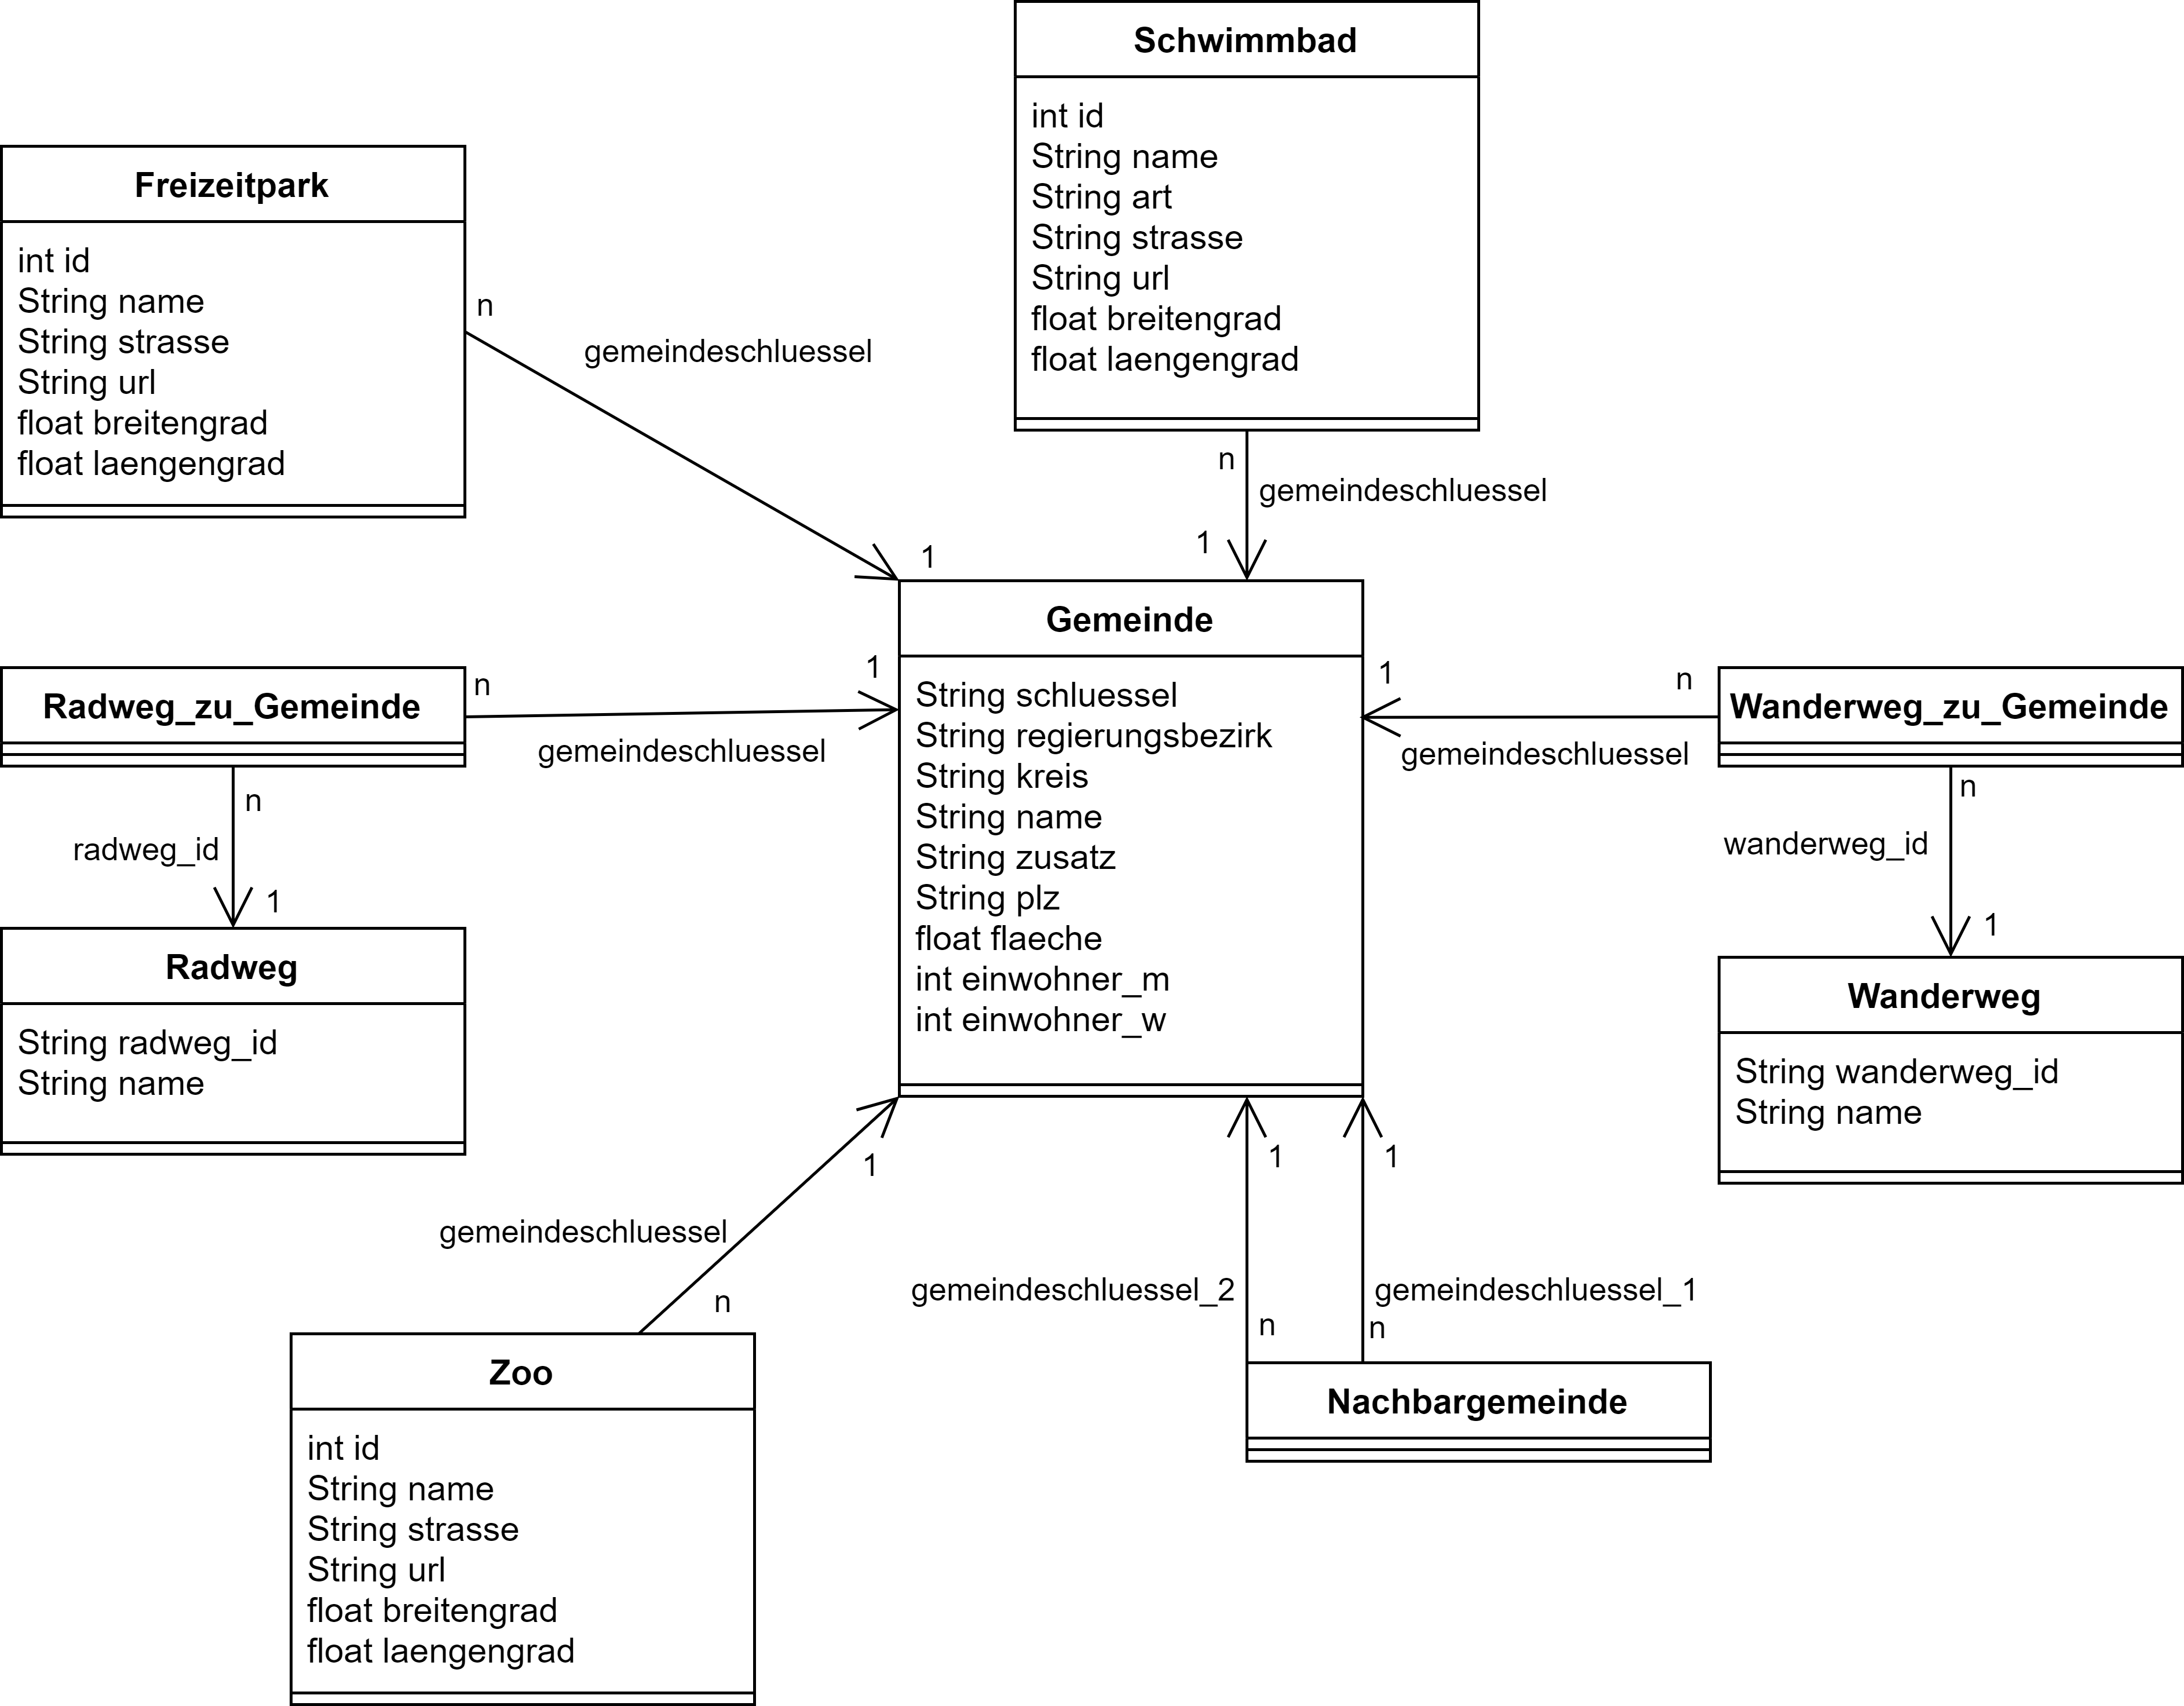
\includegraphics[width=\textwidth]{Aufgaben/img/Bayern_DB.png}
\end{center}

\Aufgabe{Aufgaben}{

Alle Aufgaben beziehen sich auf die Datenbank oben. Eine Online-Version gibt es unter \url{www.dbiu.de/bayern/}.

Gib immer genau die geforderten Daten aus und nicht mehr. Sortiere nicht, wenn du nicht dazu aufgefordert wirst.

\vspace{1cm}


Verändere die SQL-Abfrage so, dass die Namen und Internetadressen (=url) aller Zoos und der Name und Regierungsbezirk der jeweiligen Gemeinde ausgegeben wird:

\vspace{0.3cm}

\large
\emphBlue{SELECT Zoo.name, Gemeinde.name} \LoesungLuecke{,Gemeinde.regierungsbezirk, Zoo.url}{8cm}\\\vspace{0.5cm}
\emphBlue{FROM Zoo, Gemeinde}\\
\LoesungLuecke{WHERE Zoo.gemeindeschluessel = Gemeinde.schluessel}{17cm}
}


\vspace{0.3cm}


Verändere die SQL-Abfrage so, dass die der Namen und Straßen aller Freizeitparks und die Namen der jeweils zugehörigen Gemeinde ausgegeben wird.

\vspace{0.3cm}
\large
\emphBlue{SELECT Freizeitpark.name, Gemeinde.name} \LoesungLuecke{, Freizeitpark.strasse}{8cm}\\\vspace{0.5cm}
\emphBlue{FROM Freizeitpark, Gemeinde}\\
\LoesungLine{WHERE Gemeinde.schluessel = Freizeitpark.gemeindeschluessel}{1}


\vspace{0.3cm}


Schreibe eine SQL-Abfrage, die Namen und Art aller Schwimmbäder und den Namen und alle Einwohnerzahlen der zugehörigen Gemeinden ausgibt.

\LoesungLine{SELECT Schwimmbad.name, Schwimmbad.art, \\ Gemeinde.name, Gemeinde.einwohner\_m, Gemeinde.einwohner\_w\\
FROM Schwimmbad, Gemeinde\\
WHERE Gemeinde.schluessel = Schwimmbad.gemeindeschluessel}{4}


\vspace{0.3cm}


Schreibe eine SQL-Abfrage, die die Anzahl an Schwimmbädern in Gemeinden mit \emph{mehr} als 1000 weiblichen Einwohnerinnen ausgibt.

\emph{Tipp: Hier brauchst du mehrere verknüpfte Bedingungen}

\LoesungLine{SELECT COUNT(*)\\
FROM Schwimmbad, Gemeinde\\
WHERE Gemeinde.schluessel = Schwimmbad.gemeindeschluessel\\
  AND Gemeinde.einwohner\_w > 1000}{4}




\vspace{0.3cm}


Schreibe eine SQL-Abfrage, die die Namen aller Gemeinde in Oberbayern oder Niederbayern, zu denen ein Wanderweg führt, ausgibt. Dopplungen dürfen auftreten und sollte nicht entfernt werden!

\emph{Tipp: Hier brauchst du wieder mehrere verknüpfte Bedingungen. Überlege bei der Verknüpfung von Bedingungen, ob du Klammern setzen musst!}

\LoesungLine{SELECT Gemeinde.name\\
FROM Gemeinde,Wanderweg\_zu\_Gemeinde\\
WHERE Gemeinde.schluessel = Wanderweg\_zu\_Gemeinde.gemeindeschluessel\\
AND (Gemeinde.regierungsbezirk='Oberbayern' \\
OR Gemeinde.regierungsbezirk='Niederbayern')}{5}


\vspace{0.3cm}


Schreibe eine SQL-Abfrage, die aus den Tabellen Gemeinde und Wanderweg\_zu\_Gemeinde die Anzahl der Wanderwege, die zu Gemeinden mit mehr als 500 000 männlichen Einwohnern führen, ausgibt.


\LoesungLine{SELECT COUNT(*)\\
FROM Gemeinde, Wanderweg\_zu\_Gemeinde\\
WHERE Gemeinde.schluessel = Wanderweg\_zu\_Gemeinde.gemeindeschluessel\\
  AND einwohner\_m > 500000}{4}


\vspace{0.3cm}


Schreibe eine SQL-Abfrage, die eine Liste mit den Namen aller Gemeinden, die ein "Freibad" haben, und die Namen der jeweiligen Freibäder ausgibt. 

\LoesungLine{SELECT Gemeinde.name, Schwimmbad.name\\
FROM Gemeinde, Schwimmbad\\
WHERE Gemeinde.schluessel=Schwimmbad.gemeindeschluessel\\
AND Schwimmbad.art="Freibad"}{4}



\vspace{0.3cm}



Schreibe eine SQL-Abfrage, die die Anzahl an Radwegen, die an Gemeinden im PLZ-Bereich \emphOrange{größer} als 96400 angrenzen, ausgibt.

\LoesungLine{SELECT COUNT(*)\\
FROM Gemeinde, Radweg\_zu\_Gemeinde\\
WHERE Gemeinde.schluessel=Radweg\_zu\_Gemeinde.gemeindeschluessel\\
  AND Gemeinde.plz > 96400}{4}



\vspace{0.3cm}


\begin{minipage}[t]{\textwidth}
Schreibe eine SQL-Abfrage, die die Namen aller Zoos in einer Gemeinde namens "Erlangen" ausgibt.

\LoesungLine{SELECT Zoo.name\\
FROM Zoo,Gemeinde\\
WHERE Zoo.gemeindeschluessel = Gemeinde.schluessel\\
AND Gemeinde.name="Erlangen"}{4}
\end{minipage}



\vspace{0.3cm}



Schreibe eine SQL-Abfrage, die die IDs aller Radwege, die zu Gemeinden in Oberfranken oder Unterfranken führen, ausgibt. Dopplungen sollen nicht entfernt werden.

\LoesungLine{SELECT Radweg\_zu\_Gemeinde.radweg\_id\\
FROM Radweg\_zu\_Gemeinde, Gemeinde\\
WHERE Gemeinde.schluessel = Radweg\_zu\_Gemeinde.gemeindeschluessel\\
  AND (Gemeinde.regierungsbezirk = "Oberfranken" \\
  OR Gemeinde.regierungsbezirk="Unterfranken")}{6}

        \section*{Datenbank}

Gegen ist eine Datenbank mit folgenden Tabellenschemata:  \\\\

Freizeitpark(\underline{id:INT}, name:STRING, \dotuline{gemeindeschluessel:STRING}, strasse:STRING, url:STRING, breitengrad:FLOAT, laengengrad:FLOAT)\\

Gemeinde(\underline{schluessel:STRING}, regierungsbezirk:STRING, kreis:STRING, name:STRING, zusatz:STRING, plz:STRING, flaeche:FLOAT, einwohner\_m:INT, einwohner\_w:INT)\\

Nachbargemeinde(\dotuline{gemeindeschluessel\_1:STRING}, \dotuline{gemeindeschluessel\_2:STRING})\\

Radweg(name:STRING, \underline{radweg\_id:STRING})\\

Radweg\_zu\_Gemeinde(\dotuline{radweg\_id:STRING}, \dotuline{gemeindeschluessel:STRING})\\

Schwimmbad(\underline{id:INT}, name:STRING, art:STRING, \dotuline{gemeindeschluessel:STRING}, strasse:STRING, url:STRING, breitengrad:FLOAT, laengengrad:FLOAT)\\

Wanderweg(name:STRING, \underline{wanderweg\_id:STRING})\\

Wanderweg\_zu\_Gemeinde(\dotuline{wanderweg\_id:STRING}, \dotuline{gemeindeschluessel:STRING})\\

Zoo(\underline{id:INT}, name:STRING, \dotuline{gemeindeschluessel:STRING}, strasse:STRING, url:STRING, breitengrad:FLOAT, laengengrad:FLOAT)\\


\section*{Aufgabe 1}







\begin{minipage}[t]{\textwidth}
Schreibe eine SQL-Abfrage, die die Namen aller Zoos in einer Gemeinde namens "Erlangen" ausgibt.

\LoesungLine{SELECT Zoo.name\\
FROM Zoo,Gemeinde\\
WHERE Zoo.gemeindeschluessel = Gemeinde.schluessel\\
AND Gemeinde.name="Erlangen"}{4}
\end{minipage}


\vspace{0.3cm}

Schreibe eine SQL-Abfrage, die die Anzahl an Radwegen, die an Gemeinden im PLZ-Bereich \emphOrange{größer} als 96400 angrenzen, ausgibt.

\LoesungLine{SELECT COUNT(*)\\
FROM Gemeinde, Radweg\_zu\_Gemeinde\\
WHERE Gemeinde.schluessel=Radweg\_zu\_Gemeinde.gemeindeschluessel\\
  AND Gemeinde.plz > 96400}{4}




\begin{minipage}[t]{\textwidth}
\section*{Aufgabe 2}

Zeichne das vollständige (Datentypen, Beziehungen, Kardinalitäten, alle Klassen) Klassendiagramm für diese Datenbank.


\LoesungKaro{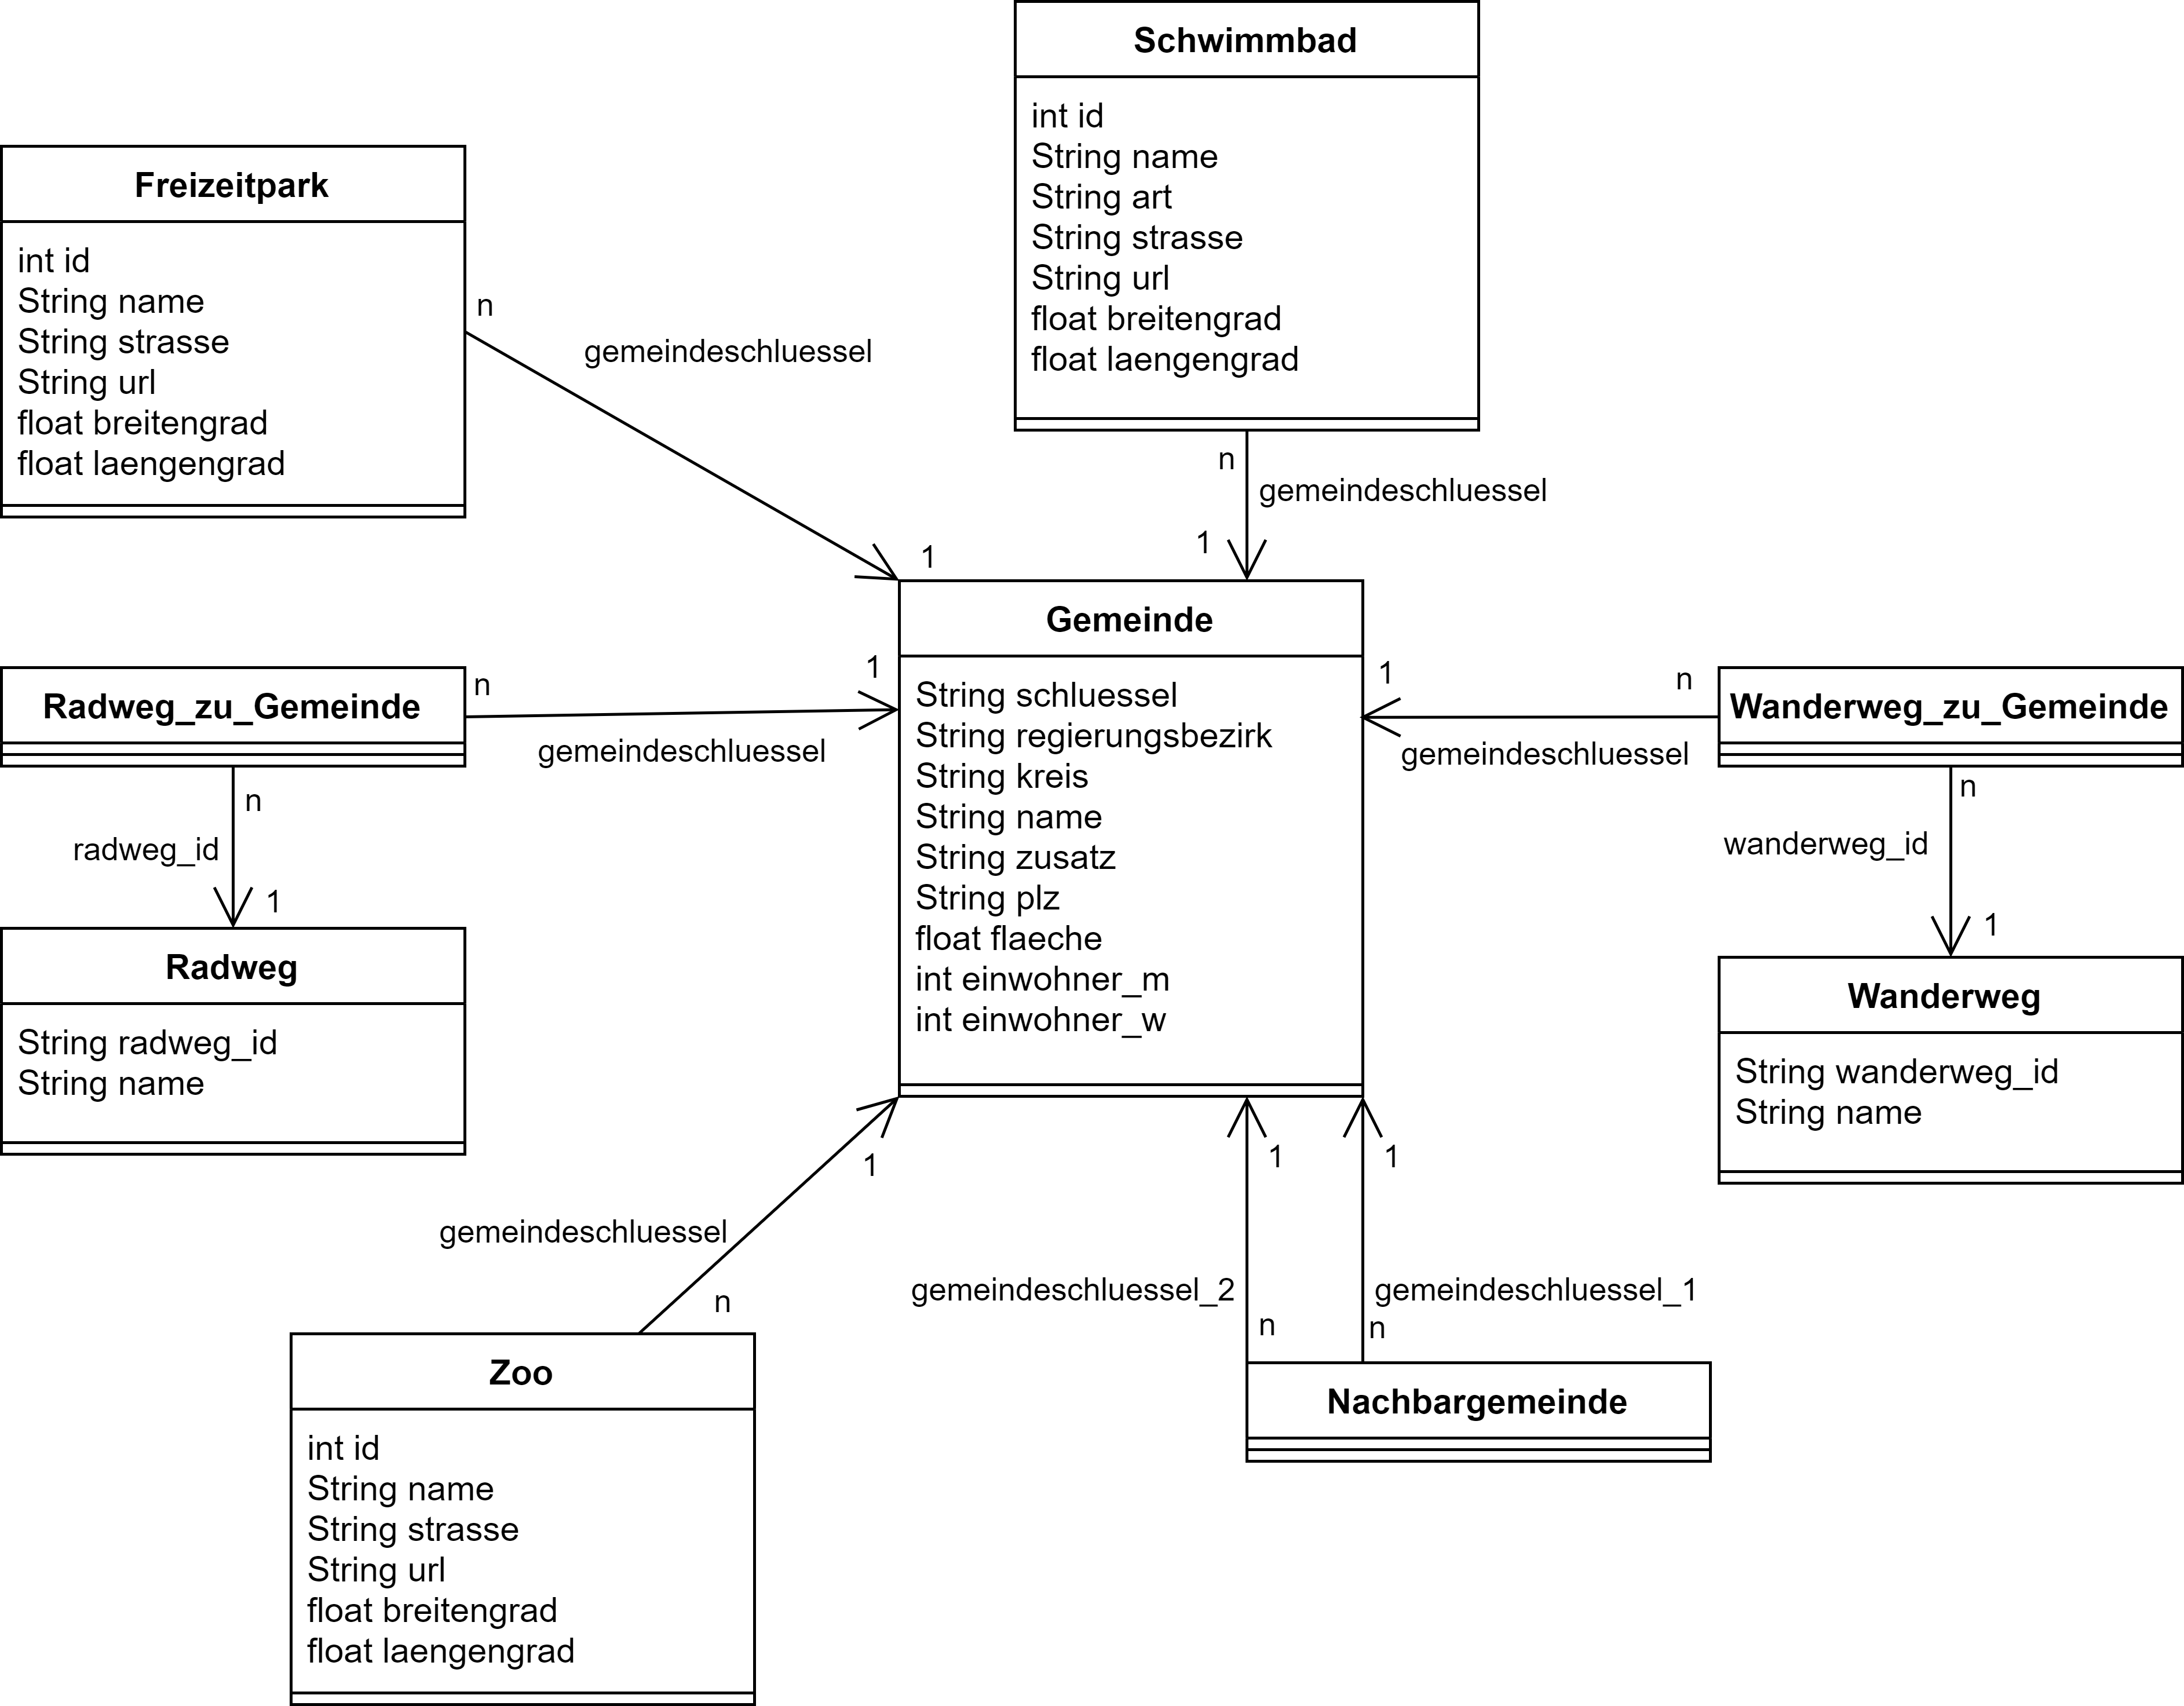
\includegraphics[width=\textwidth]{Aufgaben/img/Bayern_DB.png}}{49}
\end{minipage}

        \Aufgabe{YoungDB}

\begin{enumerate}
    \item \emphColB{Kopiere} aus dem Vorlagenordner des Ressourcen-Laufwerks (\emphColB{R:/gy0187/klassen/10x/Vorlagen/}) die Datei \emphColB{YoungDB.exe} in dein \emphColB{Laufwerk H:/}  (alternativ als Download: \url{klassenkarte.de/index.php/tools/youngdb/})
    \item Öffne nun das Programm YoungDB mit einem Doppelklick auf \emphColB{YoungDB.exe}.
    \item Lege ein \emphColB{neues Datenbankmodell an und speichere es} auf deinem Laufwerk H:/. Dieses kann mit einem Klick auf \emph{Modell speichern unter} gespeichert werden und mit \emph{Modell laden} wieder geöffnet werden.\\\\
    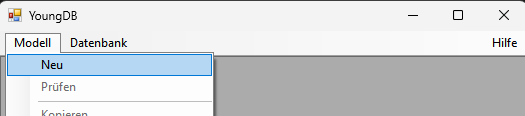
\includegraphics[width=0.4\textwidth]{img/YDB_ModellNeu.png}
    \item Lege \emphColB{zwei neue Klassen} an, bearbeite sie mit \emph{Doppelklick} und erstelle jeweils einen \emphColB{ganzzahligen Primärschlüssel id}.\\\\
    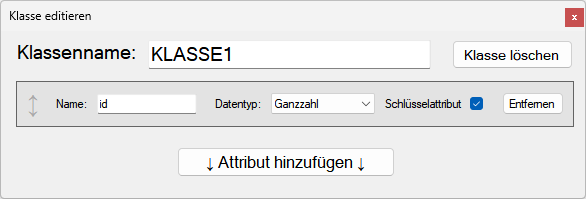
\includegraphics[width=0.5\textwidth]{img/YDB_idErstellen.png}
    \item Erstelle eine Beziehung zwischen den beiden Klassen, indem du mit \emph{Rechtsklick, Halten und Ziehen} eine rote Linie aus einer der Klassen zur anderen ziehst und dann die Maus loslässt. Bearbeite die Beziehung anschließend mit \emph{Doppelklick}, sodass sie eine \emphColB{1:n Beziehung von Klasse2 zu Klasse1} ist.\\\\
    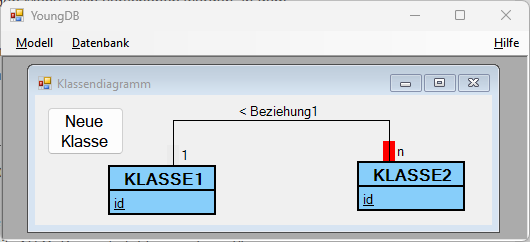
\includegraphics[width=0.5\textwidth]{img/YDB_1nBeziehung.png}\\
    \emph{Tipp:} Klassen kannst du per Doppelklick und \emph{Klasse löschen} entfernen und eine Beziehung, indem du den roten Kasten, der erscheint, wenn deine Maus am Anfang der Linie ist, irgendwo hin ziehst.
    \item \emphColB{Beantworte:} Welche Unterschiede stellst du zu normalen Klassendiagrammen fest?\\\LoesungLine{keine Datentypen, }{2}
    \item Erstelle aus dem Modell eine \emphColB{neue Datenbank und speichere sie} auf deinem Laufwerk H:/. Verwende einen ähnlichen Namen wie für das Modell.Hier kannst du Tabellen öffnen, Daten eintragen, SQL-Abfrage schreiben, speichern und laden.\\\\
    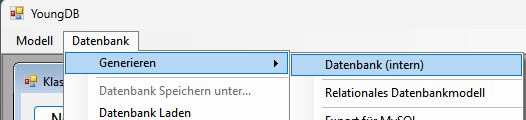
\includegraphics[width=0.45\textwidth]{img/YDB_dbGenerieren.png}
\end{enumerate}





        \Aufgabe{m:n-Beziehungen}

\begin{enumerate}
    \item Erstelle in YoungDB ein Datenbankmodell mit den Klassen Lehrkraft und Schulklasse, die in einer m:n-Beziehung zueinander stehen. Überlege dir sinnvolle Primärschlüssel und 1-2 Attribute und eine sinnvolle Bezeichnung für die Beziehung.
    \item Generiere nun die zugehörige Datenbank und befülle die Tabellen mit jeweils 2-3 Datensätzen.
    \item Beantworte folgende Fragen:\begin{itemize}
        \item Welchen essentiellen Unterschied gibt es zwischen m:n-Beziehungen und 1:n-/1:1-Beziehungen?\\
        \LoesungLine{Beziehungstabelle benötigt}{1}
        \item Was für Datensätze werden in der dritten Tabelle eingetragen?\\
        \LoesungLine{Paare von IDs der Datensätze der anderen Tabellen, die in Beziehung zueinander stehen}{2}
        \item Welche Spalten welcher Tabelle(n) sind Fremdschlüssel?\\\LoesungLine{beide Spalten der dritten Beziehungstabelle}{1}
        \item Welche Spalte(n) sind Primärschlüssel in der dritten Tabelle? \emph{Tipp: Was muss eindeutig sein? Probiere deine Vermutung aus, indem du versucht mehrere Datensätze mit gleichem (vermuteten) Primärschlüssel einzufügen.} 
        \\\LoesungLine{beide Spalten zusammen}{1}
        \item Ist es sinnvoll bei m:n-Beziehungen im Klassendiagramm eine Richtung anzugeben und wieso?
        \\\LoesungLine{}{2}
        \item Wie könnte man m:n-Beziehung im Klassendiagramm alternativ darstellen?
        \\\LoesungLine{zusätzliche Beziehungstabelle mit zwei 1:n-Beziehungen}{1}
        \item Zeichne die Darstellung von m:n-Beziehungen in YoungDB ein:\\\\
        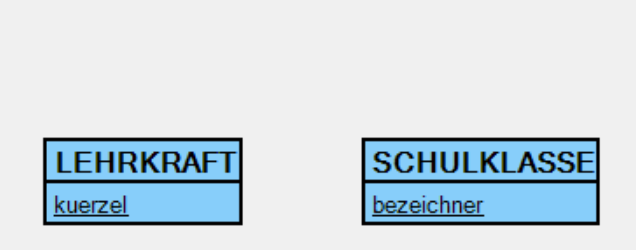
\includegraphics[width=0.6\textwidth]{Aufgaben/img/YDB_lehrerKlasse.png}
    \end{itemize}
\end{enumerate} 

        \Hefteintrag{1.9}{Darstellung von m:n-Beziehungen}{

m:n-Beziehungen können im UML-Klassendiagramm auf zwei verschiedene Arten dargestellt werden:
\vspace{0.5cm}

\emphOrange{1. \LoesungLuecke{als direkte Beziehung}{15cm}}\\
Vorteil: \LoesungLuecke{Diagramm kompakt und übersichtlich}{15cm}

\vspace{0.5cm}
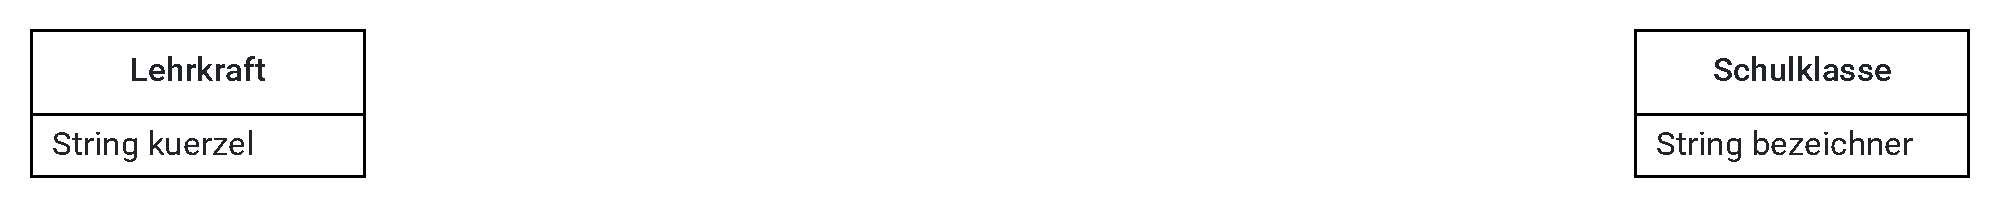
\includegraphics[width=\textwidth]{Aufgaben/img/mn-Beispiel}


\emphOrange{2. \LoesungLuecke{mit Beziehungstabelle}{15cm}}\\
Vorteil: \LoesungLuecke{Diagramm kompakt und übersichtlich}{15cm}

\vspace{1.5cm}
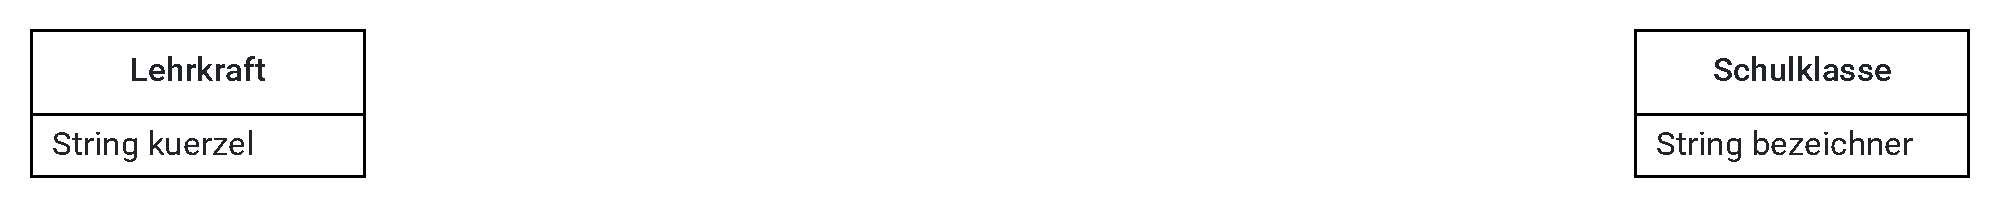
\includegraphics[width=\textwidth]{Aufgaben/img/mn-Beispiel}\\

}

        \Hefteintrag{1.9}{SQL-Abfragen mit Join bei m:n-Beziehungen}{
Um zwei Tabellen, die eine m:n-Beziehung miteinander haben, zu joinen (also ihren Join zu bilden und in der Ergebnistabelle nur \LoesungLuecke{zusammengehörende}{7cm} Datensätze zu haben), muss man:
\begin{itemize}
    \item Daten aus allen \LoesungLuecke{drei}{2cm} Tabellen abfragen (also diese nach \emphOrange{\LoesungLuecke{FROM}{3cm}} auflisten).
    \item Die \emphOrange{\LoesungLuecke{Beziehungstabelle}{8cm}} einzeln mit den normalen Tabellen joinen. Hierfür benötigt man \emphOrange{\LoesungLuecke{zwei}{2cm}} Join-Bedingungen, die mit \emphOrange{\LoesungLuecke{AND}{2cm}} verknüpft werden.
\end{itemize}

\emphOrange{Beispiel:}

\emphGreen{SELECT} Lehrkraft.*, Schulklasse.*\\
\emphGreen{FROM} Lehrkraft, Schulklasse, \emphBlue{\LoesungLuecke{Lehrer\_unterricht\_Klasse}{10cm}}\\
\emphGreen{WHERE} \emphBlue{Lehrer\_unterricht\_Klasse.lehrer} = \LoesungLuecke{Lehrkraft.kuerzel}{8cm} \\
\emphGreen{AND}  \emphBlue{Lehrer\_unterricht\_Klasse.klasse} = \LoesungLuecke{Schulklasse.bezeichner}{8cm}

}


        \begin{minipage}[t]{\textwidth}
\Aufgabe{Song-Datenbank Diagramme: \url{www.dbiu.de/songs}}

Zeichne die \emphColB{Klassenkarten} der Tabellen und \emphColB{Song und Playlist}. Zeichne anschließend mit \emphColC{zwei verschiedenen Farben} die beiden \emphColC{Darstellungsmöglichkeiten der Beziehung} zwischen den beiden Tabellen ein.

\LoesungKaro{\includegraphics[width=0.5\textwidth]{img/07_Songs.png}}{13}\\
    
\end{minipage}

        %\Aufgabe{Song-Datenbank SQL}

Bearbeite dann folgende SQL-Aufgaben auf der Website \url{www.dbiu.de/songs} und notiere die getesteten Abfragen. 


\begin{enumerate}
    
    %\item  Welche Songs (alle Attribute) gibt es insgesamt?\\
    %\LoesungLine{SELECT * FROM Song}{1}
    
    %\item Welche IDs haben die Songs, die in irgendeiner Playlist enthalten sind?\\
    %\LoesungLine{SELECT Song.id FROM Song, Song\_in\_Playlist WHERE Song\_in\_Playlist.song\_id = Song.id}{2}
    
    \item Welche Songs (alle Attribute) sind in irgendeiner Playlist enthalten?\\
    \LoesungLine{SELECT Song.* 
    FROM Song, Song\_in\_Playlist 
    WHERE Song\_in\_Playlist.song\_id = Song.id}{2}
    
    \item Gib die Titel aller Playlists und die Titel der jeweils zugehörigen Songs aus.\\
    \LoesungLine{SELECT Playlist.titel, Song.titel
    FROM Song, Playlist, Playlist, Song\_in\_Playlist 
    WHERE Song\_in\_Playlist.song\_id = Song.id 
    AND Song\_in\_Playlist.playlist\_id = Playlist.id}{4}

    \item Welche Songs (alle Attribute) sind in der Playlist namens 'Fussballhits' enthalten?\\
    \LoesungLine{SELECT Song.* 
    FROM Song, Song\_in\_Playlist, Playlist 
    WHERE Song\_in\_Playlist.song\_id = Song.id 
    AND Song\_in\_Playlist.playlist\_id = Playlist.id
    AND Playlist.tiel = 'Fussballhits'}{5}
\end{enumerate}
    }
}